\documentclass{article}

\usepackage{../preamble}
\standalonetrue

\pagestyle{fancy}
\fancyhf{}
\rhead{Section \thesection}
\lhead{MATH 316 Lecture 19}
\rfoot{Page \thepage}


\title{MATH 316 Lecture 19}
\author{Ashtan Mistal}
\date{June 16, 2021}

\begin{document}

\ifstandalone
\maketitle
\fi

\graphicspath{{./Lecture19/}}


last time, we did:

\begin{itemize}
    \item Examples on BVPs
    \item S-L problem including C-E equations
    \begin{itemize}
        \item For solving Laplace's equation (inhomogeneous BC on $\theta$)
    \end{itemize}
\end{itemize}

\textbf{GO THROUGH YESTERDAYS NOTES.  THERE ARE MORE THINGS ADDED. CHECK CANVAS. }

\section{Examples}

\subsection{Continuing example 28}

Laplace Equation, where $u(r, \alpha) = f(r)$

$$u(r, \theta) = \sum_{n=1}^\infty B_n \sinh (\mu_n \theta) \sin (\mu_n \ln r)$$

$$u(r, \alpha) = f(r) = \sum_{n=1}^\infty B_n \sinh (\mu_n \alpha) \sin (\mu_n \ln r)$$

When we have an S-L function, use the formula given (during June 14th lecture):

\begin{equation}
\label{orthogonality relation}
b_n = \frac{\int_0^\ell r(x) f(x) \phi_n (x) dx}{\int_0^\ell r(x) \phi_n^2 (x) dx}
\end{equation}



We found that $b_n = \frac{2}{\ln(2)} \int_1^2 \frac{1}{r} f(r) \sin(\mu_n \ln r) dr = \frac{2}{\ln(2)} \int_1^2 \frac{1}{r} \sin (\mu_n \ln(r)) dr$

Take $f(r) = 1$. To do the integral we set $ln(r) = u$ and $\frac{dr}{r} = du$

$$b_n^{f(S-L)} = \frac{2}{ln(2)} \int_0^{\ln(2)} \sin(\mu_n u) du = \frac{2}{\ln(2)} \left[ - \frac{1}{\mu_n} \cos (\mu_n u) \right]_0^{\ln(2)} = \frac{-2}{\ln(2)} \frac{2 \ln 2}{(2n-1) \pi} \left[ \cos( \mu_n \ln(2)) - 1 \right]$$

$$ = \frac{4}{(2n-1)}$$

Finally, we have the following:

$$u(r, \theta) = \frac{4}{\pi} \sum_{n=1}^\infty \frac{1}{(2n-1)} \frac{\sinh(\mu_n \theta)}{\sinh(\mu_n \frac{\pi}{2})} \sin (\mu_n \ln(r))$$

For $n = 1$, 

$$\mu_1 = \frac{\pi}{2 \ln(2)} \to u_1(r, \theta) = \frac{4}{\pi} \frac{\sinh(\frac{\pi}{2 \ln 2} \theta)}{\sinh( \frac{\pi}{2 \ln 2} \frac{\pi}{2})} \sin \left( \frac{\pi}{2 \ln 2} \ln r \right)$$

Let's fix $\theta = \theta_1$. Then, $u_1(r, \theta) = \underbrace{K}_{\text{constant}} \cdot \sin \left( \frac{\pi}{2 \ln 2} \ln(r) \right)$

\begin{center}
    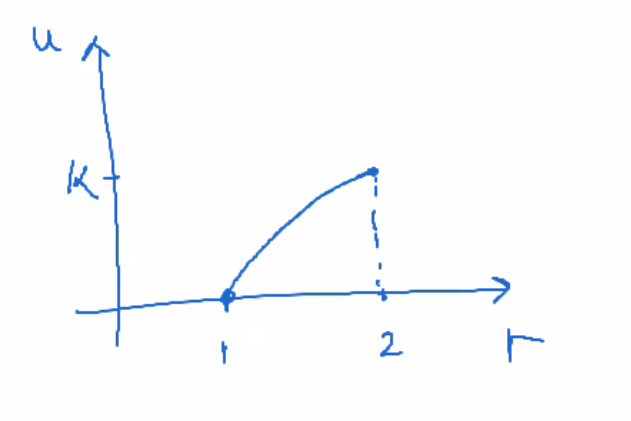
\includegraphics[width = 0.6 \textwidth]{1.png}
\end{center}

\section{Heat Equation with Robin Boundary Conditions}

NOTE: one way to find a more general S-L problem, compared to the eigenvalue problems we saw previously in the heat, wave, and Laplace's equation with Dirichlet or Neumann boundary conditions, is to make the boundary conditions more general. 

\subsection{Example 29}

Assume a steel beam subjected to a fire on one end. 

\begin{center}
    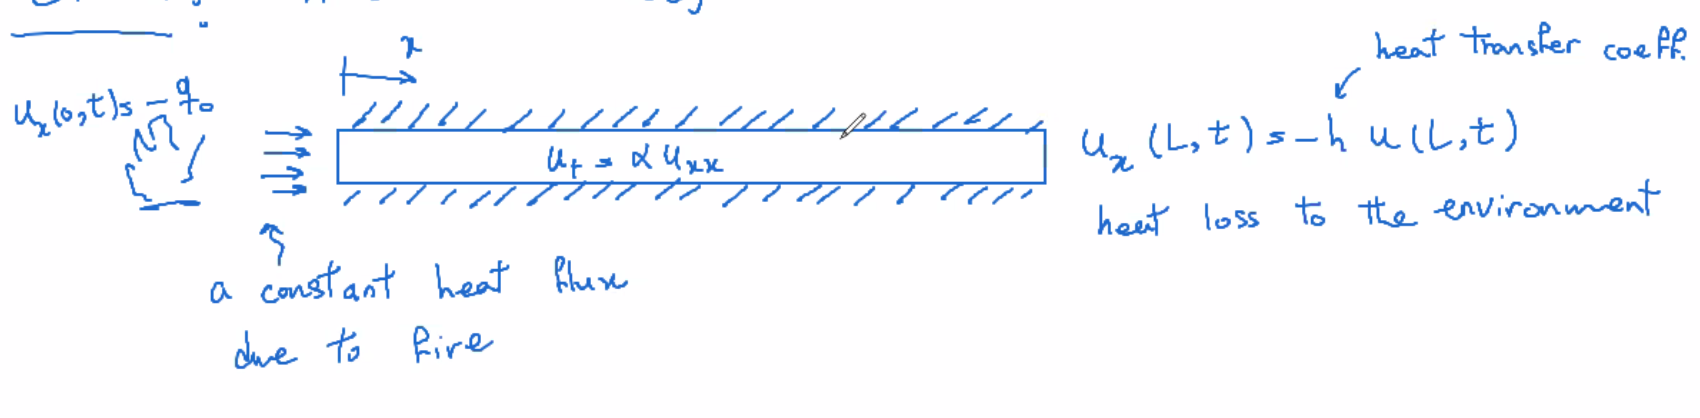
\includegraphics[width = 0.95 \textwidth]{2.png}
\end{center}

$u_t = \alpha u_{xx} \quad 0 < x < L, t > 0$

$\underbrace{u_x(0,t) = - q_o}_{\text{Inhomogeneous}} (1) \quad u_x(L,t) = -h u(L,t) (2)$

IC: $u(x,0) = f(x)$

We need to remove the inhomogeneous boundary condition first. We need to separate solution into a steady state and a transient part: $u(x,t) = w(x) + v(x,t)$

\hfill

Steady state: $W(x) = Ax + B$. Subbing in the first boundary condition gives us $w=(0) = -q_0 = A$. Plugging in the second we get that $w'(L) = -h w(L)$. This gives us $- q_0 = -h (- q_0 L + b)$. As a result, $B = \frac{q_0}{h} + q_0 L$.

Therefore the steady state solution is the following:

$$w(x) = - q_0 x + \frac{q_0}{h} + q_0 L$$

\hfill

Transient part:

$v_t = \alpha^2 v_{xx}$. 

Boundary conditions: $u_x (0,t) = w_x(0) + v_x(0,t) = - q_0 \Rightarrow v_x(0,t) = 0$

$u_x(L,t) = - h u(L,t) \longrightarrow w_x(L) + v_x(L,t) = - h (w(L) + v(L,t))$. We know that $w_x(L) = - q_0$ and therefore $- q_0 + v_x(L,t) = - h \left( - q_0 L + \frac{q_0}{L} + q_0 L \right) - h v(L,t)$

Hence, $v_x(L,t) = - h V (L,t)$

Using the initial conditions, $u(x,0) = f(x)$

$w(x) + v(x,0) = f(x) \longrightarrow v(x,0) = f(x) - w(x)$

We therefore solve this using separation of variables:

$$\frac{X''}{X} = \frac{\dot{T}}{\alpha T} = - \lambda$$

BVP: $X'' + \lambda X = 0$

$X'(0) = 0$ and $X'(L) = - h X(L)$

This is an S-L BVP (similar to example 26). 

$\lambda = \mu^2 > 0$

$$X(x) = A \cos(\mu x) + B \sin(\mu x)$$

Given $X'(L) = -h X(L)$, $- A \mu \sin(\mu L) = - h A \cos(\mu L) \Rightarrow \tan(\mu_n L) = \frac{h}{\mu_n}$ for $n \in \NN$

$$X'(x) = -A \mu \sin(\mu x) + B \mu \cos(\mu x)$$

Given $X'(0) = 0$, $B = 0$

Plot $tan(x)$ and $\frac{1}{x}$, and find intersections as $\mu_n$. 

$\Rightarrow \mu_n \approx \frac{n \pi}{L}, \quad x_n = \cos(\mu_n x)$ (Eigenvalues and eigenfunctions respectively)

\hfill

Now, we move on to the IVP:

$$\frac{\dot{T_n}}{T_n} = - \alpha \lambda_n \Rightarrow T_n = e^{- \alpha \mu_n^2 t}$$

Finally we superimpose the solution:

$$v(x,t) = \sum_{n=0}^\infty A_n e^{- \alpha \mu_n^2 t} \cos(\mu_n x)$$

To find $a_n$, we apply $v(x,0) = f(x) - w(x) = \sum_{n=0}^\infty A_n \cos(\mu_n x)$

Using the orthogonality relation for S-L eigenfunctions (\ref{orthogonality relation}):

$r(x) = 1$

$$A_n = \frac{\int_0^\ell (f(x) - w(x)) \cos(\mu_n x) dx}{\int_0^\ell r(x) \cos^2 (\mu_n x) dx}$$

$$\int_0^L \cos^2 (\mu_n x) dx = \int_0^L \frac{1}{2} \left\{ 1 + \cos(2 \mu_n x) \right\} dx = \frac{1}{2} \left\{ \left. x \right|_0^L + \frac{1}{2 \mu_n} \left. \sin \left( 2 \mu_n x \right) \right|_0^L \right\}$$

$$ = \frac{1}{2} \left\{ L + \frac{1}{2 \mu_n} \sin(2 \mu_n L) \right\} = \frac{1}{2} \left\{ L + \frac{1}{\mu_n} \sin(\mu_n L) \cos(\mu_n L) \right\}$$

We find that $\mu_n = \frac{h}{\tan(\mu_n L)}$

and hence:

$$= \frac{1}{2} \left\{ L + \frac{\sin^2 (\mu_n L) \cos(\mu_n L)}{h \cos(\mu_n L)} \right\} = \frac{1}{2} \left\{ L + \frac{\sin^2 (\mu_n L)}{h} \right\}$$

Therefore:

$$A_n = \frac{2 \int_0^\ell (f(x) - w(x)) \cos(\mu_n x) dx}{L + \frac{\sin^2(\mu_n L)}{h}}$$

Finally:

$$u(x,t) = w(x) + v(x,t) = - q_0 x + \frac{q_0}{h} + q_0 L + \sum_{n=0}^\infty A_n e^{- \alpha \mu_n^2 t} \cos (\mu_n x)$$

NOTE: As $t \to \infty$, $u(x,t) = w(x)$. 

\begin{center}
    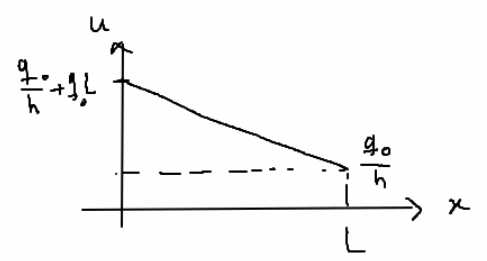
\includegraphics[width = 0.6 \textwidth]{3.png}
\end{center}

\subsection{Example 30: Robin BCs on both ends}

The heat equation with robin boundary condition on both ends. 

$u_t = \alpha u_{xx} \quad 0 
< x < L, \quad t > 0$

BC: $u_x(0,t) = u(0,t), \quad u_x (L,t) = - u(L,t)$

IC: $u(x,0) = f(x)$

Solution: Separation of variables. 

$$\frac{X''}{X} = \frac{\dot{T}}{\alpha T} = - \lambda$$

BVP:

$$X'' + \lambda X = 0$$

$$X'(0) = X(0)$$

$$X'(L) = - X(L)$$

Hence we have $\lambda = \mu^2 > 0$ and therefore we have the solution:

$$X(x) = A \cos(\mu x) + B \sin(\mu x)$$

$$X'(x) = - A \mu \sin(\mu x) + B \mu \cos(\mu x)$$

From the first boundary condition, $B \mu = A$


From the second BC, $(- A \mu + \frac{A}{\mu} \sin(\mu L) = (-A - A) \cos(\mu L)$

Therefore, $\tan(\mu L) = \frac{2 \mu}{\mu^2 - 1}$ ($\mu = 1$ is a singular point)

This can be solved numerically: (Plotting $L = 1$ for simplicity)

\begin{center}
    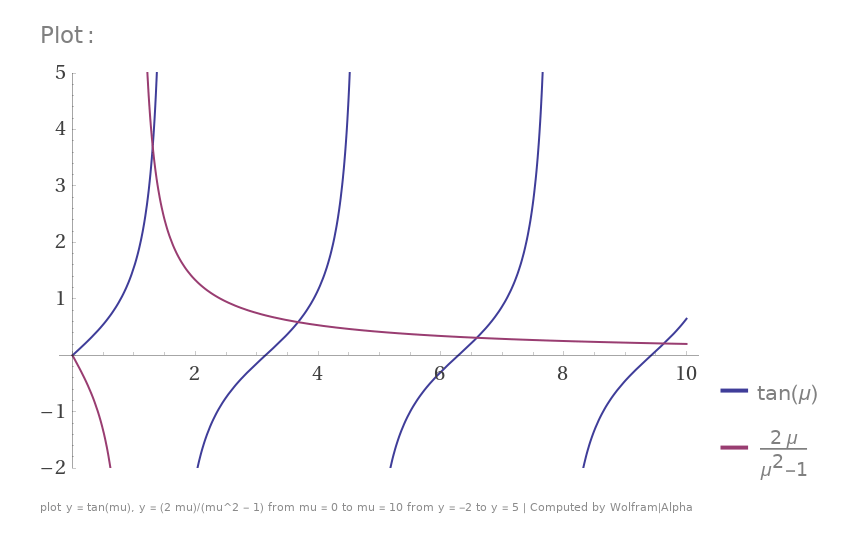
\includegraphics[width = 0.9 \textwidth]{7.png}
\end{center}

$$X_n(x) = \mu_n \cos(\mu_n x) + \sin(\mu_n x)$$

\hfill

Next, we need to solve the IVP:

If $L = 1$: $\mu_0 \approx 1.3, \mu_1 \approx 3.63, \mu_2 \approx 6.55, \mu_3 \approx 9.56$. AS $n \to \infty, \mu_n \to n \pi$

$$T_n = e^{- \alpha \mu_n^2 t}$$

Hence

$$u(x,t) = \sum_{n=1}^\infty A_n e^{- \alpha \mu_n^2 t} \left( \mu_n \cos(\mu_n x) + \sin(\mu_n x) \right)$$

When do we sum from $n = 1$ as opposed to $n = 0$? When $n = 0$ gives us a trivial solution (such as with Robin BCs), we do not include it in the sum as it is the wrong approach (even if mathematically correct). 

From inhomogeneous BCs we find $A_n$.  and substitute $A_n$ into $u(x,t)$. 


\section{Non-homogeneous Sturm - Liouville  problems}

The general format is in the form of

\begin{equation}
\label{general format}
    \mathcal{L} y = - \left( p(x) y' \right)' + q(x) y = \underbrace{\mu}_{\text{constant}} r(x) y + \underbrace{f(x)}_{\text{note}}
\end{equation}


note: A given function on $0 \leq x \leq 1$. 

Boundary conditions:

$$\left\{ \begin{matrix} \alpha_1 y(0) + \alpha_2 y'(0) = 0 \\ \beta_1 y(1) + \beta_2 y'(1) = 0 \end{matrix} \right.$$

We need to use the Fredholm Alternative Theorem (Find theorem in module week 6). 

The results of the Fredholm Alternative Theorem says the following:

\begin{itemize}
    \item If $\mu = \lambda$ (eigenvalues of the homogeneous S-L problem), then \ref{general format} need not have a solution for every $f(x)$, even if it happens to have a solution, the solution is not unique. 
    \item If $\mu \neq \lambda$, then equation \ref{general format} has a unique solution for $f(x)$. 
\end{itemize}

This theory only tells us if a unique solution exists. 

\subsection{Solving nonhomogenous S-L BVP: Example 31}

\begin{itemize}
    \item Decompose $f(x)$ and $y(x)$ in terms of the eigenfunctions of the homogeneous problem. Then, solve for the coefficients of the series for $y(x)$.  
\end{itemize}

EX 31: Solve the BVP:

$$y'' + 4y = x, \quad x \in (0, \frac{\pi}{2})$$

$$y(0) = 0, y'(\frac{\pi}{2}) = 0$$

Solution:

$$y'' + \lambda y = 0, y(0) = 0, \quad y'(\frac{\pi}{2}) = 0$$

This is a homogeneous S-L as we have seen before. Hence, $\lambda_n = (2n-1)^2$ for $n \in \NN$, and $y_n = \sin((2n-1) x)$

$\mu = -4 \neq (4n-1)^2$ according to the Fredholm alternative, there is a unique solution for this problem. Hence we write $f(x) = x$ as:

$$f(x) = x = \sum_{n=1}^\infty b_n \sin \left( (2n-1) x \right)$$

$$b_n = \frac{4}{\pi} \int_0^{\pi/2} x \sin \left( (2n-1) x \right) dx = \frac{4}{\pi} \frac{(-1)^{n+1}}{(2n-1)^2}$$

Then we write:

$$y(x) = \sum_{n=1}^\infty d_n \sin \left( (2n-1) x \right)$$

Then, we plug in $f(x)$ and $y(x)$ in the BVP: 

$$y'' + 4y = x$$

$$\sum_{n=1}^\infty \left( 4 - (2n-1)^2 \right) d_n \sin \left( (2n-1) x \right) = \frac{4}{\pi} \sum_{n=1}^\infty  \frac{(-1)^{n+1}}{(2n-1)^2} \sin \left( (2n-1) x \right)$$

$$d_n = \frac{4}{\pi} \frac{(-1)^{n+1}}{(2n-1)^2} \frac{1}{4 - (2n-1)^2}$$

$$\therefore y(x) = \sum_{n=1}^\infty \frac{4}{\pi} \frac{(-1)^{n+1} \sin((2n-1) x)}{(2n-1)^2 \left( 4 - (2n-1)^2 \right)}$$







\end{document}